\documentclass[hidelinks,a4paper,12pt]{article}
\usepackage[left=2in, right=1in, top=1in, bottom=1in]{geometry}
\usepackage[table]{xcolor}
\usepackage{graphicx}
\usepackage{sectsty} %to customise headings
%\usepackage{attachfile}
%\usepackage{navigator}
\usepackage{times} %this is for the selection of font
%\usepackage[english]{babel} %this is for the selection of font
%\usepackage{Palatino}
%\usepackage{courier}
%\usepackage[T1]{fontenc}
%\renewcommand*\familydefault{\ttdefault} %% Only if the base font of the document is to be typewriter style
\usepackage{float}
\usepackage{fancyhdr}	
\usepackage[ampersand]{easylist}
\usepackage{amssymb}
\usepackage{enumitem}	
\usepackage{caption} \captionsetup[table]{singlelinecheck=false, margin=1em}
%\usepackage{tabu}
\usepackage{longtable}
\usepackage{booktabs}
\usepackage{eso-pic}
%\usepackage{transparent}
\usepackage{pdfpages}

\usepackage{ltablex}
\setlength{\LTpre}{0pt}
\setlength{\LTpost}{-15pt}

\usepackage{array}
\usepackage{tabularx}


\usepackage{pgfplots, pgfplotstable}
%\usepackage{makecell}
\usetikzlibrary{backgrounds}
% background color definition from pgfmanual-en-macros.tex
\definecolor{graphicbackground}{cmyk}{0,0,0,.03}
% key to change color
\pgfkeys{/tikz/.cd,
	background color/.initial=graphicbackground,
	background color/.get=\backcol,
	background color/.store in=\backcol,
}
\tikzset{background rectangle/.style={
		fill=\backcol,
	},
	use background/.style={    
		show background rectangle
	}
}
	
\pagestyle{fancy}
\fancyhf{}
\lhead{Project Synopsis}
\rhead{\textbf { \textsl{Service Request to a Cloud}}}
\lfoot{\scriptsize{MCS-44 Mini Project\\IGNOU Enrollment ID : 137132696\\ }}
% Set the right side of the footer to be the page number
\cfoot{}

\renewcommand{\headrulewidth}{0.4pt}
\renewcommand{\footrulewidth}{0.4pt}

%\usepackage{lipsum}% Used for dummy text.

\definecolor{titlepagecolor}{cmyk}{1,.60,0,.40}
\definecolor{namecolor}{cmyk}{0.4,.2,0.,.10} 
\definecolor{levelfirst}{cmyk}{0,0,0,0.70}
\definecolor{levelSecond}{cmyk}{1,.50,0,.10}
\definecolor{levelthird}{cmyk}{1,.50,0,.10}
\definecolor{levelfourth}{cmyk}{1,.50,0,.10}
\definecolor{levelfifth}{cmyk}{1,.50,0,.10}

\definecolor{tablecell1}{cmyk}{0.07,0.03,0.03,0.07}
\definecolor{tablecell2}{cmyk}{0.04,0.02,0.02,0.04}

\sectionfont{\fontsize{16}{22}\selectfont}
\subsectionfont{\fontsize{14}{18}\selectfont}
\subsubsectionfont{\fontsize{12}{16}\selectfont}
%\renewcommand{\abstractnamefont}{\fontsize{16}{22}\selectfont \bfseries}
%\renewcommand{\abstracttextfont}{\normalfont}

%-----------------------------------------------------------------
\begin{document}

\begin{titlepage}

\thispagestyle{empty}
\pagenumbering{roman}

\vspace{0.25in}
\hspace{-1.5in}
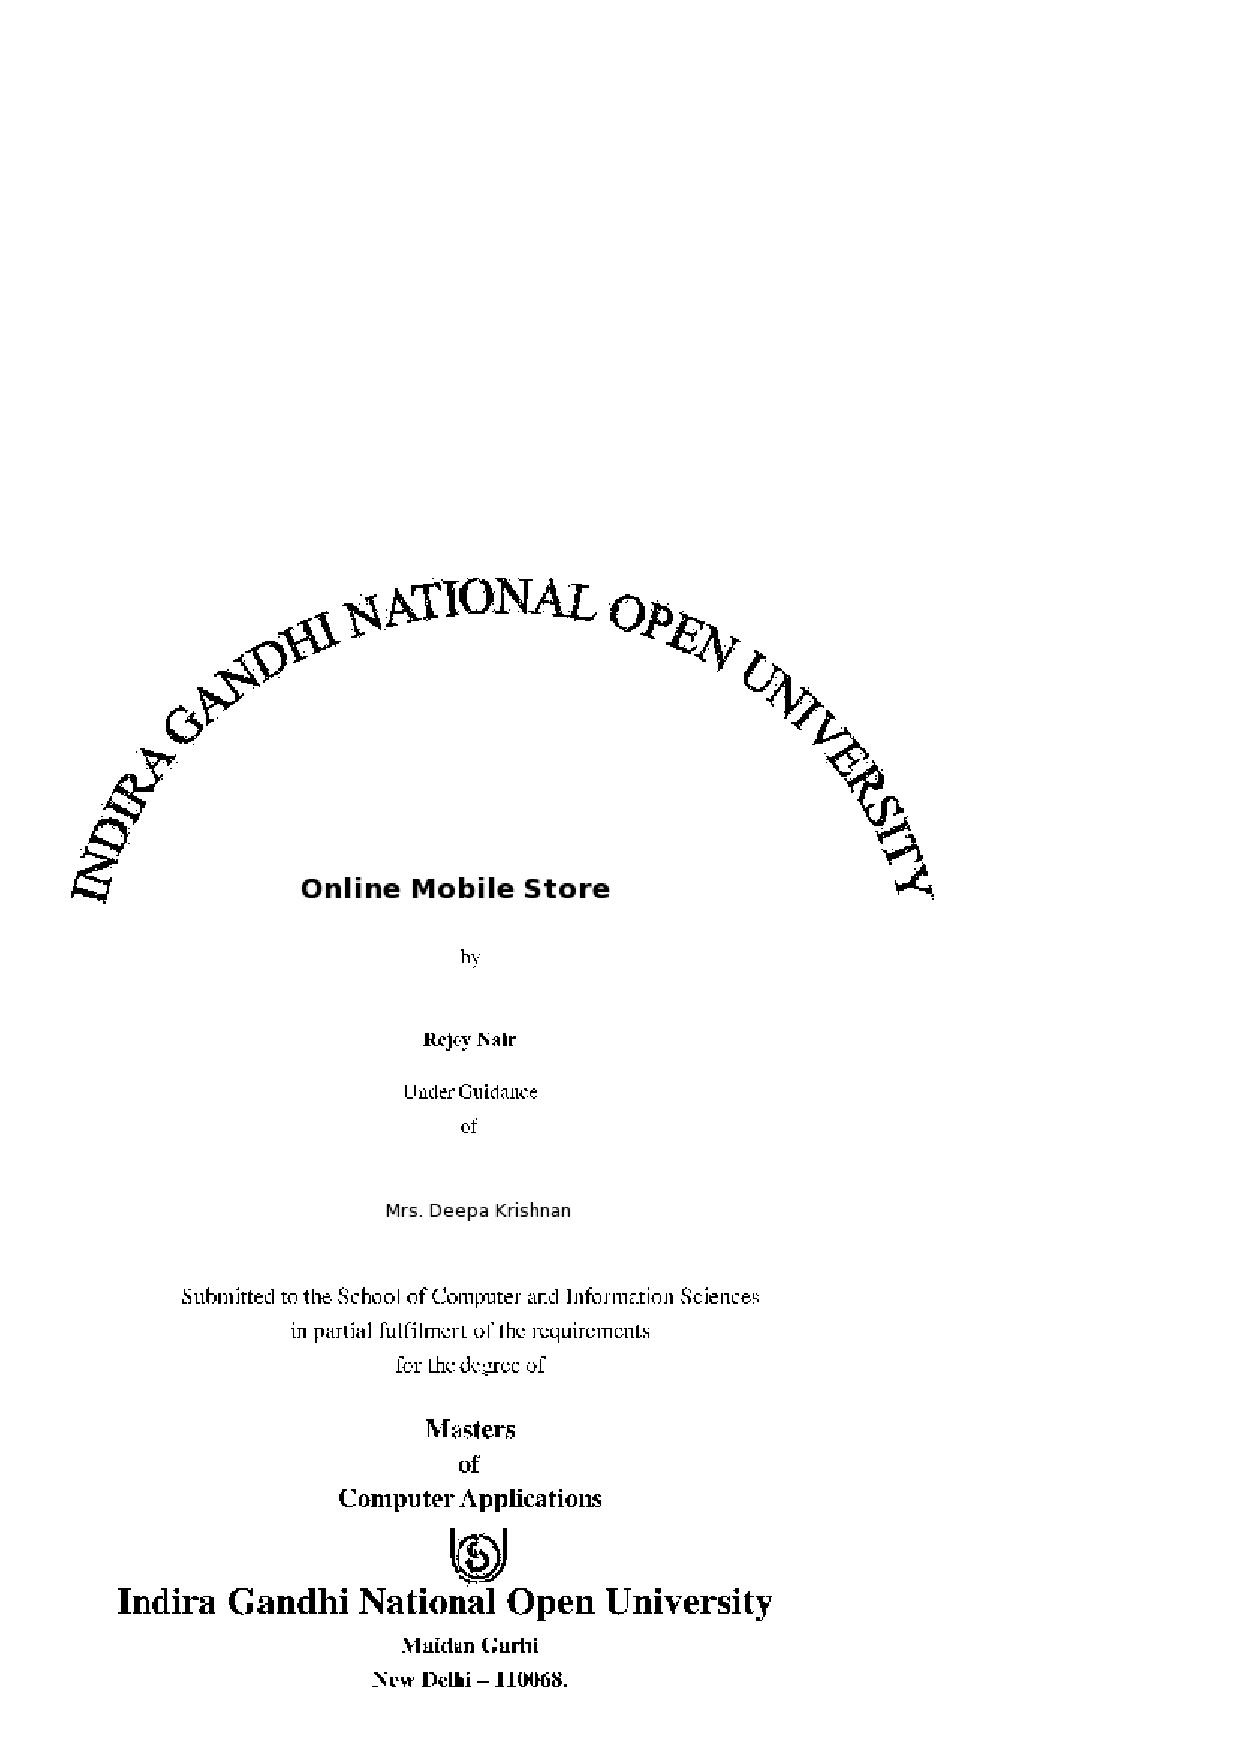
\includegraphics[ width={0.88\paperwidth} , keepaspectratio ]{Titlepage1.png} \\
\vfill
\end{titlepage}
	
\newpage
\pagestyle{plain}
\pagenumbering{roman}
\setcounter{page}{2}

\hspace{-1.5in}
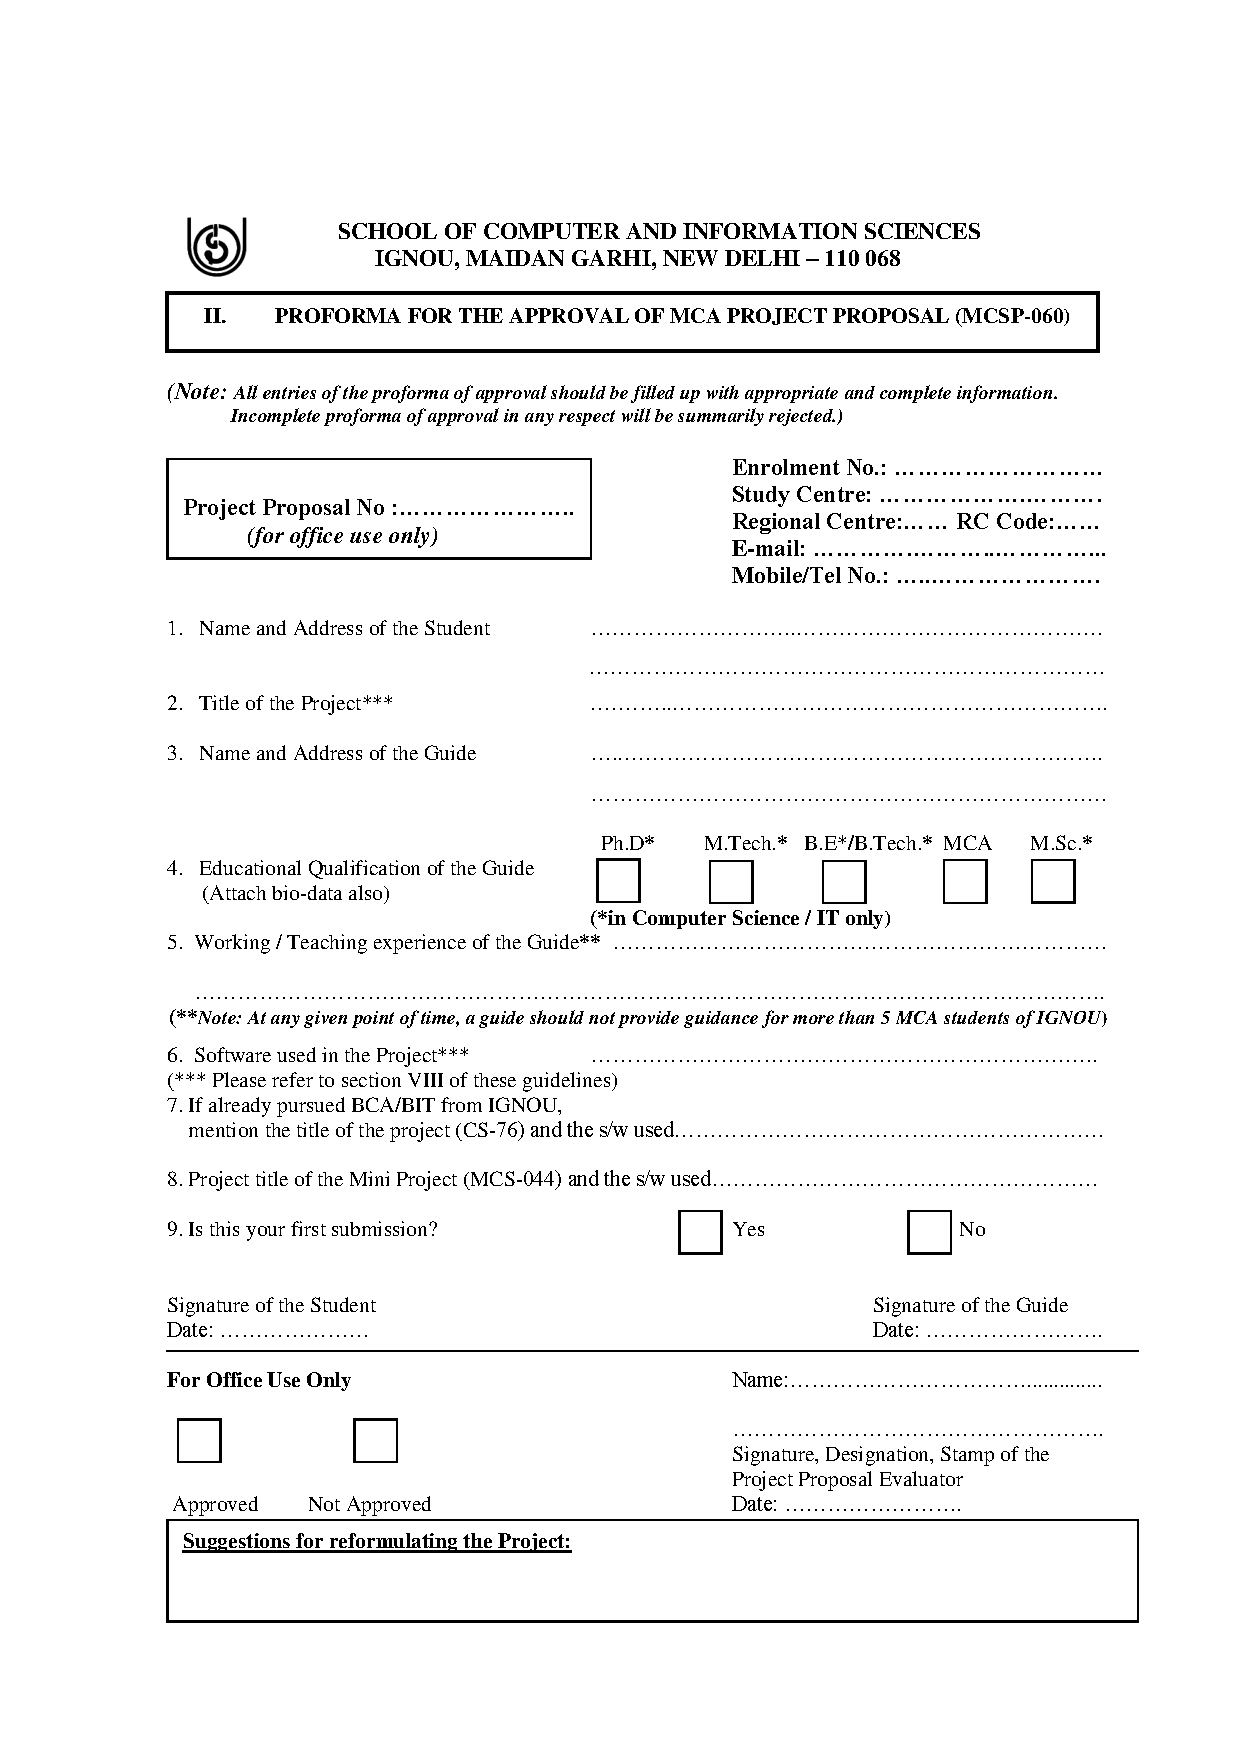
\includegraphics[ height={0.81\paperheight} , keepaspectratio ]{outputproforma.png} \\
\vfill

\iffalse{
\newpage

\begin{center}
\hspace{-1.5in}
\textbf {CERTIFICATION} \\
\end{center}

\hspace{-1.5in}

\includegraphics[ width={0.9\paperwidth} , keepaspectratio ]{pg3.eps}\\
\vfill
}
\fi

\newpage
	
\tableofcontents
	
\setcounter{tocdepth}{3}
	
	
\newpage

\clearpage

\pagestyle{plain}
\setcounter{page}{1}
\pagenumbering{arabic}
%\fancyfoot[R]{\thepage}


\section{Introduction}
Electronic commerce commonly written as E-commerce or ecommerce is the trading or facilitation of trading using computer networks such as Internet or Social Networks. Electronic Commerce draws on technologies such as mobile commerce, electronics funds transfer, supply chain management, Internet Marketing, Online Transaction Processing, Electronic Data Interchange (EDI), inventory management systems and automated data collection systems. Modern electronic commerce typically uses the world wide web for atleast one part of the transaction's life cycle although it may also use other technologies like email.
\\

Online Shopping is a from of electronic commerce which allows consumers to directly buy good or services from a seller over the internet using a web browser. Consumers find a product of interest by visiting the website of the retailer directly or by searching among alternative vendors using a shopping search engine which displays the same product's availablity and pricing at different vendors. Customers can shop online using a range of different computers and devices including desktop computers, laptops, tablet computers and smartphones.
\\

In this synopsis high-level details of implementation of an Online Mobile Store will be provided.
\bigskip

\newpage


\subsection{Background}
An online shop evokes the physical analogy of buying products and services at a regular "bricks-and-mortar" retailer or shopping center; the process is called business-to-consumer (B2C) obline shopping. A typical online store enables the customer to browse the firm's range of products and services, view photos or images of the products, along with information about the product specifications, features and prices.
\\

Online stores typically enable shoppers to use "search" features to find specific models, brands or items. Online customers must have access to the Internet and a valid method of payment in order to complete a transaction, such as a credit card, an Interac-enabled debit card, or a service such as PayPal. For physical products (e.g., paperback books or clothes), the e-tailer ships the products to the customer; for digital products, such as digital audio files of songs or software, the e-tailer typically sends the file to the customer over the Internet. The largest of these online retailing corporations are Alibaba, Amazon.com, and eBay
\\

English entrepreneur Michael Aldrich was a pioneer of online shopping in 1979\textsuperscript{[1]}. His system connected a modified domestic TV to a real-time transaction processing computer via a domestic telephone line.The first World Wide Web server and browser, created by Tim Berners-Lee in 1990, opened for commercial use in 1991.Thereafter, subsequent technological innovations emerged in 1994: online banking, the opening of an online pizza shop by Pizza Hut, Netscape's SSL v2 encryption standard for secure data transfer, and Intershop's first online shopping system. The first secure retail transaction over the Web was either by NetMarket or Internet Shopping Network in 1994.Immediately after, Amazon.com launched its online shopping site in 1995 and eBay was also introduced in 1995. Alibaba's sites Taobao and Tmall were launched in 2003 and 2008 respectively.
\\

Mobile Phone online buying platforms can be broadly classified into 2 types\\

\ListProperties(Hide=100, Hang=true, Progressive=6ex, Space=0.8em,Space*=0.8em, Style*=$\bullet$, Style2*=$\bullet$ ,Style3*=$\bullet$ ,Style4*=\tiny$\blacksquare$ )

\begin{easylist}
& \thinspace Owned by Retailer to sell own products 
& \thinspace Marketplace, which allows various merchants to showcase and sell their products. The retailer only manages the marketplace.
\end{easylist}

\bigskip

This project initially focuses on the implementation of a platform which the retailer can use to sell own products i.e the retailer is accountable and responsible for the product inventory.

\noindent
\subsubsection {Purpose and Motivation}

The main purpose of this project is to create an online store to buy mobile phones. The site will allow users to search mobile phone based on a set of features. Users can add the selected products to a shopping cart and checkout by making payment. Users will receive an order copy of their invoice.
\\

The retailer website will be managed by an Admin. Admin will have additional functionality such as managing product catalouge and generating reports.
\\

Motivation to work on this project includes

\ListProperties(Hide=100, Hang=true, Progressive=6ex, Space=0.8em,Space*=0.8em, Style*=$\bullet$, Style2*=$\bullet$ ,Style3*=$\bullet$ ,Style4*=\tiny$\blacksquare$ )

\begin{easylist}
& \thinspace Work on a project in the Retail domain
& \thinspace Interest to find out the working of a good user friendly website that facilitates online transactions using a database
& \thinspace Interest in technologies like GOLang, CSS, HTML and SQL for web development
& \thinspace Explore data analytics that can be implemented using GOLang
\end{easylist}
\\

\bigskip

\noindent
\subsection{Objectives}

\ListProperties(Hide=100, Hang=true, Progressive=6ex, Space=0.8em,Space*=0.8em, Style*=$\bullet$, Style2*=$\bullet$ ,Style3*=$\bullet$ ,Style4*=\tiny$\blacksquare$ )

\begin{easylist}
& \thinspace Implement Admin Module for managing a website facilitating buying of mobile phones using online transactions
& \thinspace Develop and host website which allows users to search and explore mobile phones
& \thinspace Implement the Shopping Cart feature for the site that allows users to add selected products and tag it to a single order
& \thinspace Implement the Online Payment Module (Credit Cards Only)
& \thinspace Explore technologies like GOLang, CSS, HTML and SQL for web development
& \thinspace Explore data analytics that can be implemented using GOLang for Reports generation
\end{easylist}


\bigskip


\newpage

\section{Project Category}

This project can be categorised as a web development project that uses concepts of Internet technologies and web design, Web security and RDBMS. Though GOLang is not an OOPs language per se, nonetheless concepts of OOPs will be used using Interfaces allowed in GOlang. Network Security to secure the payment gateway shall be explored and implemented.

\section{Tools/Platform, Hardware \& Software Requirements}

A good e-commerce site should present the following factors to users for better usability

\ListProperties(Hide=100, Hang=true, Progressive=6ex, Space=0.8em,Space*=0.8em, Style*=$\bullet$, Style2*=$\bullet$ ,Style3*=$\bullet$ ,Style4*=\tiny$\blacksquare$ )

\begin{easylist}
& \thinspace Simple navigation from home page to information and order links for specific
products.
& \thinspace Obvious shopping links or buttons.
& \thinspace Effective categorical organization of products.
& \thinspace Easy scanning and selecting items in a list.
& \thinspace Consistent layout of product information.
& \thinspace Minimal and effective security notifications or messages.
& \thinspace Knowing when an item was saved or not saved in the shopping cart.
& \thinspace Returning to different parts of the site after adding an item to the shopping cart.
\end{easylist}

\bigskip
\noindent

To deploy a website with the basic benchmarks as stated above the following tools, platforms , hardware and software are being considered.
\\

The development environment shall be set up on a i686 computer loaded with a 32-bit Linux Operating System 
The host environment shall also be the same i686 computer with the 32-bit Linux Operating System i.e the development machine and host server are one and the same machine.

\newpage

\\
\noindent
	\begin{center}
				
		%\bigskip
							
		{
		\setlength{\extrarowheight}{2pt}
						
							
		\newcolumntype{b}{X}
		\newcolumntype{s}{>{\hsize=.4\hsize}X}
		\newcolumntype{t}{>{\hsize=1.3\hsize}X}
		
		\renewcommand\thetable{1} 					
		\captionof{table}{ \textbf {\small {Software \& Hardware Requirements}}} \label{table:1}
		\vspace{0.25cm}
									
		\begin{tabularx}{\textwidth}{ | >{\ttfamily\raggedright\arraybackslash} s 
		  | >{\ttfamily\raggedright\arraybackslash} t 
		  | >{\ttfamily\raggedright\arraybackslash} t | }
								
		\hline
								
		{\textbf{\textcolor{black}{\large {Sr. No.} \newline}}} & {\textbf{\textcolor{black}{\large {Tools \& Technologies}}}} & \textbf{\textcolor{black}{\large {Description}}} \\
								
		\hline
		1.0 & Go ver 1.7 linux/386 & Tool for managing Go source code.Go (also commonly referred to as golang) is an open source systems programming language developed at Google  \\
	    \hline		
		2.0 & Apache2 & Web Server to develop and deploy the application  \\
	    \hline
		3.0 & PostgreSQL & Database  \\ [1em]
	    \hline
		4.0 & PGAdmin3 & Database Administration Utility  \\  [1em]
	    \hline	  
		5.0 & Emacs ver. 24.3 & Development Environment  \\ 
	    \hline	
		6.0 & go-mode & Emacs package for GOLang \\ [1em]
	    \hline	
		7.0 & React.js & Javascript library for building User Interfaces \\ [1em]
	    \hline	 
		8.0 & Github & Repository Management Cloud  \\ [1em]
	    \hline	  
		9.0 & Git & Version Control System  \\ [1em]
	    \hline
		10.0 & HTML5 & Markup Language for designing Web Pages  \\ [1em]
	    \hline	
		11.0 & CSS & Style sheet language for describing presentation of a document created using a markup language  \\ [1em]
	    \hline		    	    		    
		12.0 & Crunchbang Linux Waldorf 11.0 & Operating System   \\ 
	    \hline	    
		13.0 & stripe-go & GOlang client for Stripe API. Stripe is a Payment Gateway Service provider   \\ 
	    \hline	   	    		       	           								
		\end{tabularx}
		}
		\end{center}
						
		\noindent
						

\bigskip

\newpage

\section{Requirements and Analysis}

\subsection{Problem Definition}
A Mobile Phone Retailer requires that it presents inventory to customers online and facilitate users to search, select and place orders for mobile phones as well as make payments online.
\\
Retailer should be able to manage the platform that allows the buying of mobile phones online.

\subsection{Admin Module}
Administrator of the website can manage the product catalouge and view basic reports

\subsubsection{Manage Products}
Admin can create, edit and delete products maintained in the product catalouge. User is presented with the list managed by Admin

\subsubsection{Reports}
Admin can generate basic report of products purchased on the website

\subsection{User Module}
Users can register, login, search for products, add selected products to shopping cart and place orders after check-out

\subsubsection{Self-Registration}
User can register using email address on the website

\subsubsection{Sign-On}
User can sign-on using email address

\subsubsection{Search Products}
User can search for specific products in the search catalogue by description or by features that completely describe the product

\subsubsection{Shopping Cart}
Selected products can be added to shopping cart. Shopping Cart is not persistent i.e it is valid only for the session

\subsubsection{Place Order}
Users can trigger orders after checkout by making payment.

\subsubsection{Make Payment}
Users can use the payment gateway integrated into the website using API

\subsubsection{Invoice}
Users can receive invoice copy on their registered email addresses

\subsubsection{Notifications}
User can receive notifications regarding sign-in, selected products, payment success and order confirmation


\bigskip

\newpage

\subsection{Planning and Scheduling}

\noindent
\textbf{Major deliverables of this project are:}

\ListProperties(Hide=100, Hang=true, Progressive=6ex, Space=0.8em,Space*=0.8em, Style*=$\bullet$, Style2*=$\bullet$ ,Style3*=$\bullet$ ,Style4*=\tiny$\blacksquare$ )

\begin{easylist}
& \thinspace Setting up the development environment
& \thinspace Code implementation of the key functions i.e Product Catalogue, Sign-on, Order management \& Reports
& \thinspace Payment API Integration
& \thinspace Test Scenarios, Test Cases \& Testing
& \thinspace Deployment \& Hosting
\end{easylist}
\bigskip

\begin{center}
			
		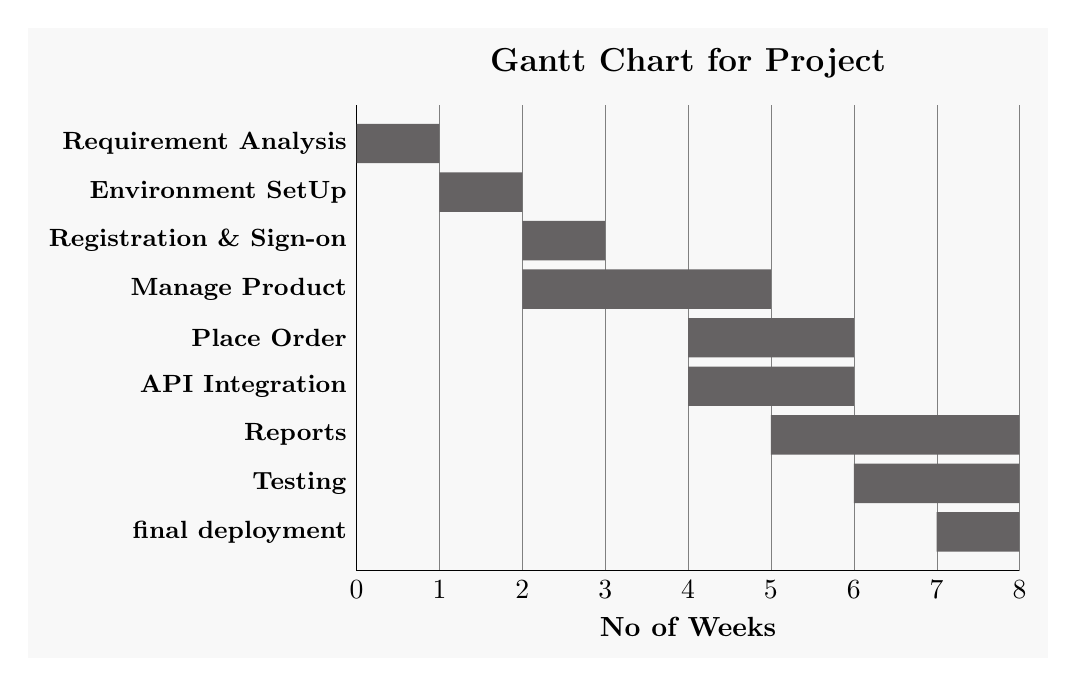
\begin{tikzpicture}[use background]
		
		\pgfplotstableread{ % Read the data into a table macro
			Label                                                      First   Second  
			{\small \textbf{final deployment}}                           7     1
			{\small \textbf{Testing}}                                    6     2
			{\small \textbf{Reports}}                                    5     3
			{\small \textbf{API Integration }}                           4     2
			{\small \textbf{Place Order}}                                4     2
			{\small \textbf{Manage Product}}                             2     3
			{\small \textbf{Registration \& Sign-on}}                    2     1
			{\small \textbf{Environment SetUp}}                          1     1
			{\small \textbf{Requirement Analysis}}                       0     1
		}\datatable
		
		\begin{axis}[
		xbar stacked,   % Stacked horizontal bars
		xmin=0,  xmax=8,       % Start x axis at 0
		title={\large \textbf {Gantt Chart for Project}},
		height=7.5cm, width=10cm,
		bar width=0.5cm,
		axis x line*=bottom,
		axis y line*=left,
		y axis line style={opacity=1},
		enlarge y limits=true,
		xmajorgrids={true},
		grid style={
			solid,
			ultra thin,
			gray
		},
		tick style={tickwidth=0cm,major tick length=0cm},
		xlabel={\textbf{No of Weeks }},
		ytick=data,     % Use as many tick labels as y coordinates
		yticklabels from table={\datatable}{Label}  % Get the labels from the Label column of the \datatable
		]
		\addplot [draw=none,fill=none] table [x=First, y expr=\coordindex] {\datatable};    % Plot the "First" column against the data index
		\addplot [draw=none,fill={levelfirst}]table [x=Second, y expr=\coordindex] {\datatable};
		
		
		\end{axis}
		

		\end{tikzpicture}
		

\end{center}
		
\noindent
These estimates may change nominally depending on the exact nature of detailed requirements.

\newpage

 

\section{Scope of the Solution}
\subsection{Purpose}
This synopsis presents the scope to implement an ``\textbf {Online Mobile Store}" 
\\

\noindent
\subsection{Scope}
This Synopsis presents high level details of functionality in the implementation of a web-based online mobile store. The current scope of the application is limited to

\ListProperties(Hide=100, Hang=true, Progressive=6ex, Space=0.8em,Space*=0.8em, Style*=$\bullet$, Style2*=$\bullet$ ,Style3*=$\bullet$ ,Style4*=\tiny$\blacksquare$ )

\begin{easylist}
& \thinspace User Registration \& Sign-on
& \thinspace Manage Products Catalogue
& \thinspace Order Management
&& Shopping Cart
&& Place Order
&& Cancel Order
& \thinspace Payment gateway integration
& \thinspace Notifications
& \thinspace Analytics \& reports

\end{easylist}
\\


\section{Analysis}

\begin{figure}[H]
\centering
\includegraphics[ width=\textwidth , keepaspectratio ]{activity-examples-online-shopping.png}\\[-1em]
\vspace{0.25cm}
\caption{Activity Diagram of Online Mobile Store}
\label{fig:2}
\end{figure}

\bigskip

\begin{figure}[H]
\centering
\includegraphics[ width=\textwidth , keepaspectratio ]{dfd1.png}\\[-1em]
\vspace{0.25cm}
\caption{Dataflow Diagram of Online Mobile Store}
\label{fig:2}
\end{figure}

\bigskip

\begin{figure}[H]
\centering
\includegraphics[ width=\textwidth , keepaspectratio ]{OrderingProcess.jpg}\\[-1em]
\vspace{0.25cm}
\caption{Ordering Process of Online Mobile Store}
\label{fig:2}
\end{figure}

\bigskip

\bigskip

\begin{figure}[H]
\centering
\includegraphics[ width=\textwidth , keepaspectratio ]{classdiagram1.jpg}\\[-1em]
\vspace{0.25cm}
\caption{Class Diagram of online shopping for Online Mobile Store}
\label{fig:2}
\end{figure}

\bigskip

\begin{figure}[H]
\centering
\includegraphics[ width=\textwidth , keepaspectratio ]{componentwebsite.png}\\[-1em]
\vspace{0.25cm}
\caption{Component Diagram for Online Mobile Store}
\label{fig:2}
\end{figure}

\bigskip

\section{Structure}

\subsection{Module Details}

\noindent
	\begin{center}
				
		%\bigskip
							
		{
		\setlength{\extrarowheight}{2pt}
						
							
		\newcolumntype{b}{X}
		\newcolumntype{s}{>{\hsize=.4\hsize}X}
		\newcolumntype{t}{>{\hsize=1.3\hsize}X}
		
		\renewcommand\thetable{2} 					
		\captionof{table}{ \textbf {\small {Modules \& Effort Estimate}}} \label{table:2}
		\vspace{0.25cm}
									
		\begin{tabularx}{\textwidth}{ | >{\ttfamily\raggedright\arraybackslash} s 
		  | >{\ttfamily\raggedright\arraybackslash} t 
		  | >{\ttfamily\raggedright\arraybackslash} t | }
								
		\hline
								
		{\textbf{\textcolor{black}{\large {Sr. No.} \newline}}} & {\textbf{\textcolor{black}{\large {Module}}}} & \textbf{\textcolor{black}{\large {Effort Estimate}}} \\
								
		\hline
		1.0 & User Registration \& Sign-On & 1 Week  \\
	    \hline		
		2.0 & Manage Products & 2 Weeks  \\
	    \hline
		3.0 & Order Management & 2 Weeks  \\ [1em]
	    \hline
		4.0 & Payment Gateway API Integration & 2 Weeks  \\  [1em]
	    \hline	  
		5.0 & Reports & 4 Weeks  \\ 
	    \hline	
   	    		       	           								
		\end{tabularx}
		}
		\end{center}
						
		\noindent
						

\bigskip



\subsection{Data Structures}

\noindent
	\begin{center}
				
		%\bigskip
							
		{
		\setlength{\extrarowheight}{2pt}
						
							
		\newcolumntype{b}{X}
		\newcolumntype{s}{>{\hsize=.4\hsize}X}
		\newcolumntype{t}{>{\hsize=1.3\hsize}X}
		
		\renewcommand\thetable{3} 					
		\captionof{table}{ \textbf {\small {Data Structure}}} \label{table:3}
		\vspace{0.25cm}
									
		\begin{tabularx}{\textwidth}{ | >{\ttfamily\raggedright\arraybackslash} s 
		  | >{\ttfamily\raggedright\arraybackslash} t 
		  | >{\ttfamily\raggedright\arraybackslash} t | }
								
		\hline
								
		{\textbf{\textcolor{black}{\large {Sr. No.} \newline}}} & {\textbf{\textcolor{black}{\large {Data Structure}}}} & \textbf{\textcolor{black}{\large {Remark}}} \\
								
		\hline
		1.0 & Boolean  &   \\ [1em]
	    \hline		
		2.0 & Character &   \\ [1em]
	    \hline
		3.0 & Floating Point &  \\ [1em]
	    \hline
		4.0 & Double &  \\  [1em]
	    \hline	  
		5.0 & Integer &   \\ [1em]
	    \hline	
		6.0 & Enumerated Type &   \\ [1em]
	    \hline	   	    		       	           				7.0 & Array &   \\ [1em]
	    \hline	
	    8.0 & Linked List &   \\ [1em]
	    \hline
		9.0 & Stack &   \\ [1em]
	    \hline    
		10.0 & Queue &   \\ [1em]
	    \hline  
		11.0 & Binary Search tree &   \\ [1em]
	    \hline 	 
		12.0 & Heap &   \\ [1em]
	    \hline	    
		\end{tabularx}
		}
		\end{center}
						
		\noindent

\bigskip

\subsection{Process logic}

\begin{figure}[H]
\centering
\includegraphics[ width=\textwidth , keepaspectratio ]{processflow1.png}\\[-1em]
\vspace{0.25cm}
\caption{Process Diagram for Online Mobile Store}
\label{fig:2}
\end{figure}


\begin{figure}[H]
\centering
\includegraphics[ width=\textwidth , keepaspectratio ]{processflow2.png}\\[-1em]
\vspace{0.25cm}
\caption{Process Diagram for Online Mobile Store}
\label{fig:2}
\end{figure}


\subsection{Implementation Methodology}

\begin{figure}[H]
\centering
\includegraphics[ width=\textwidth , keepaspectratio ]{implementation1.png}\\[-1em]
\vspace{0.25cm}
\caption{Architecture Diagram for Online Mobile Store}
\label{fig:2}
\end{figure}

\bigskip

\noindent
The website will be created using the Go programming language. The front-end user interface shall be designed in HTML5 and CSS. Versioning and Code-management shall be done using git. Code repository shall be in a Github account. PostgreSQL shall be used for the database. Stripe-go shall provide the API for the dummy payment gateway system.

\subsection{List of Reports}

\noindent
	\begin{center}
				
		%\bigskip
							
		{
		\setlength{\extrarowheight}{2pt}
						
							
		\newcolumntype{b}{X}
		\newcolumntype{s}{>{\hsize=.4\hsize}X}
		\newcolumntype{t}{>{\hsize=1.3\hsize}X}
		
		\renewcommand\thetable{4} 					
		\captionof{table}{ \textbf {\small {List of Reports}}} \label{table:4}
		\vspace{0.25cm}
									
		\begin{tabularx}{\textwidth}{ | >{\ttfamily\raggedright\arraybackslash} s 
		  | >{\ttfamily\raggedright\arraybackslash} t 
		  | >{\ttfamily\raggedright\arraybackslash} t | }
								
		\hline
								
		{\textbf{\textcolor{black}{\large {Sr. No.} \newline}}} & {\textbf{\textcolor{black}{\large {List of Reports}}}} & \textbf{\textcolor{black}{\large {Description}}} \\
								
		\hline
		1.0 & User Report  &  Registered users' details \\ [1em]
	    \hline		
		2.0 & Orders Report &  Order details \\ [1em]
	    \hline
		3.0 & Products Report &  Product Details \\ [1em]
	    \hline
	
		\end{tabularx}
		}
		\end{center}
						
		\noindent

\newpage


\section{Implementation of Security Mechanisms}

\noindent
	\begin{center}
				
		%\bigskip
							
		{
		\setlength{\extrarowheight}{2pt}
						
							
		\newcolumntype{b}{X}
		\newcolumntype{s}{>{\hsize=.4\hsize}X}
		\newcolumntype{t}{>{\hsize=1.3\hsize}X}
		
		\renewcommand\thetable{5} 					
		\captionof{table}{ \textbf {\small {Security Mechanisms}}} \label{table:5}
		\vspace{0.25cm}
									
		\begin{tabularx}{\textwidth}{ | >{\ttfamily\raggedright\arraybackslash} s 
		  | >{\ttfamily\raggedright\arraybackslash} t 
		  | >{\ttfamily\raggedright\arraybackslash} t | }
								
		\hline
								
		{\textbf{\textcolor{black}{\large {Sr. No.} \newline}}} & {\textbf{\textcolor{black}{\large {Security Mechanism}}}} & \textbf{\textcolor{black}{\large {Description}}} \\
								
		\hline
		1.0 & Firewall  &   a technological barrier designed to prevent unauthorized or unwanted communications between computer networks or hosts \\ [1em]
	    \hline		
		2.0 & SSL Certificate &  Digital certificate for Secure Sockets Layer (SSL) authentication \\ [1em]
	    \hline
		3.0 & Secure Checkout &  Using stripe.js or checkout.js over https. HTTPS is a protocol for secure communication over a computer network which is widely used on the Internet. \\ [1em]
	    \hline
	
		\end{tabularx}
		}
		\end{center}
						
		\noindent

\bigskip

\section{Future Scope and further enhancement of Project}

The project can be worked upon to add more functionality to offer a better buying experience such as recommender engines and in the creation of an e-commerce website that can be deployed in the real world.

\section{Bibliography}

\scriptsize {
[1] https://en.wikipedia.org/wiki/Michael\_Aldrich
\\

\noindent



\end{document}	
	









